\documentclass{beamer}
\usepackage[latin1]{inputenc}
\usetheme{Warsaw}
\usecolortheme{wolverine}
\title{Soldering Workshop}
\author{Clint Grimsley clint.grimsley@gmail.com}
\institute{HackRVA}
\date{August 13, 2012}
\begin{document}

\begin{frame}
\titlepage
\end{frame}

\begin{frame}
  \frametitle{Outline}
    \tableofcontents
\end{frame}

\section{Methods}
\begin{frame}
\frametitle{Plated Through-Hole}
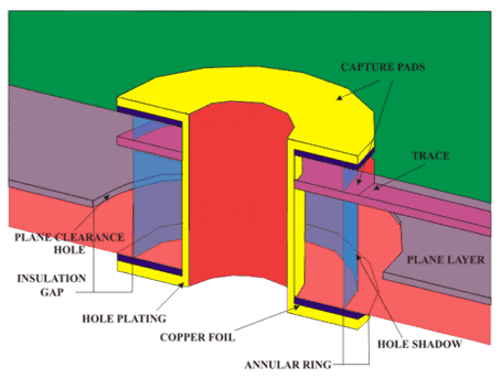
\includegraphics[scale=0.45]{images/pth.png}
\end{frame}

\begin{frame}
\frametitle{Surface Mount}
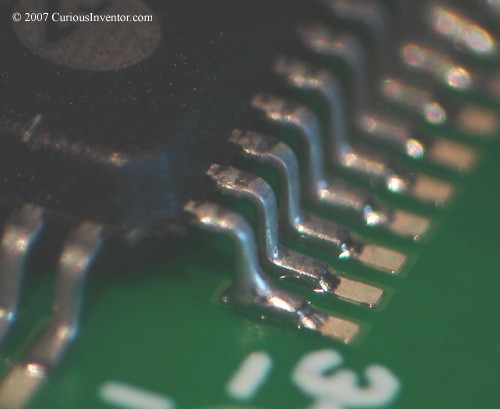
\includegraphics[scale=0.50]{images/surface_mount.jpg}
\end{frame}

\section{Solder Types}
\subsection{Tin/Lead}
\begin{frame}
  \frametitle{Sn / Pb}
  \begin{itemize}
  \item Tin (Sn)
  \item Lead (Pb)
  \item Common Combinations
    \begin{itemize}
    \item 63/37 Melting Point: 183\textdegree C (361\textdegree F)
    \item 60/40 Melting Point: Between 183-190\textdegree C (361-374\textdegree F)
    \item 50/50 Melting Point: Between 185-215\textdegree C (365-419\textdegree F)
    \end{itemize}
  \item So... It's hot. Burn cream and antiseptic are available. But please exercise CAUTION!
  \item Meaning: Point the business end of the iron at the business
    and pay attention while you're working
  \end{itemize}
\end{frame}

\begin{frame}
  \frametitle{Isn't breathing this crap bad for me?}
  \begin{itemize}
    \item Yes
    \item Use proper ventilation (we do)
    \item Take regular breaks (Once an hour is usually enough)
    \item Go outside, walk around
    \item Particluate masks are available for those that are really worried.
  \end{itemize}
\end{frame}

\section{Look and Feel}
\subsection{Good}
\begin{frame}
  \frametitle{Good}
  \begin{columns}
    \begin{column}{5cm}
      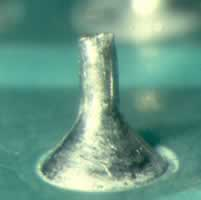
\includegraphics{images/good_joint.jpg}
    \end{column}
    \vspace{3cm}
    \begin{column}{5cm}
      \begin{itemize}
        \item Conical Shape
        \item No cold gaps
        \item Silvery vs. Gray color indicates not too much resin as to make a cold joint
      \end{itemize}
    \end{column}
  \end{columns}
\end{frame}

\subsection{Bad}
\begin{frame}
  \frametitle{Bad}  
  \begin{columns}
    \begin{column}{5cm}
      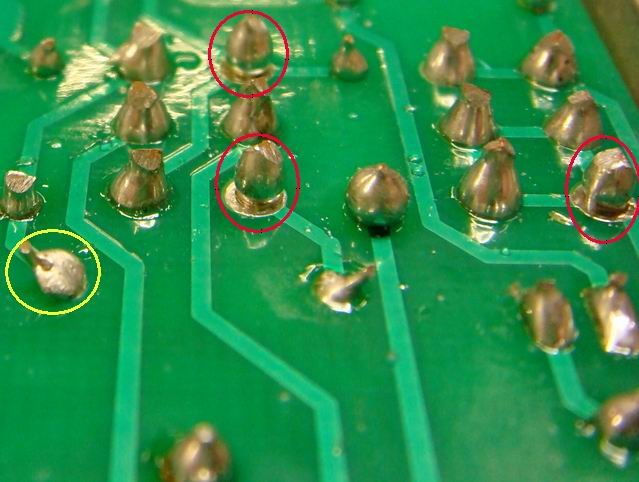
\includegraphics[scale=0.25]{images/bad_joint.jpg}
    \end{column}
    \vspace{3cm}
    \begin{column}{5cm}
      \begin{itemize}
      \item This guy is fired
      \item Notice the bulging joins, possibly not even attached to
        collector pad
      \item The yellow circle indicates there is way too much flux in
        the connection
      \end{itemize}
    \end{column}
  \end{columns}  
\end{frame}

\begin{frame}
  \frametitle{Here's how I do it}
  Watch and learn
\end{frame}

\section{History}
\begin{frame}
  \frametitle{History}
  \begin{itemize}
    \item First evidence 4000 BC
    \item historically used to make jewelry and weapons
      \begin{itemize}
      \item bling + killing the other guy = good times
      \end{itemize}
    \item Not sure who invented the electric soldering iron
    \item a few lay claim online, but they're all manufacturers,
      claiming their founders created the first electric soldering
      iron
    \item I love history, but finding this Marconi seems like a waste
      of time
    \item Further reading for those that are interested can be found
      here:
      \url{http://answers.google.com/answers/threadview?id=441944}
  \end{itemize}
\end{frame}

\section{References}

\begin{frame}
  These docs and their authors rock, and this presentation would have
  sucked more without them.
  \begin{itemize}
    \item \url{http://www.ami.ac.uk/courses/topics/0170_wsp/index.html}
    \item \url{http://pages.csam.montclair.edu/~west/phys240/Soldering.pdf}
  \end{itemize}
\end{frame}


\end{document}
